\chapter{Harmonic Motion}
\label{chapter:harmonic-motion}

In Chapter~\ref{chapter:energy}, we studied several oscillatory systems using
the law of conservation of energy, shown in ~\ref{fig:shm-systems}. But it is
clear that the law of conservation of energy does not tell us \emph{why} the
masses oscillate.
\begin{figure}[ht]
  \centering
  \begin{subfigure}{.32\textwidth}
    \centering
    \begin{tikzpicture}[scale=.85]
      \draw[mass] (3,.5) rectangle +(1,1);
      \draw[thick,
        decoration={aspect=.3,segment length=6, amplitude=2.5mm, coil},
        decorate] (0,1)--(3,1);
      \fill[pattern=north east lines] (4.3,0.5)--(4.3,.3)--(-.2,.3)
      --(-.2,2)--(0,2)--(0,.5)--cycle;
      \draw[very thick] (0,2)--(0,.5)--(4.3,.5);
    \end{tikzpicture}
    \caption{Horizontal spring-mass system}
  \end{subfigure}
%    \begin{displaymath}
%      K+U_e=\text{constant}
  %    \end{displaymath}
  \hspace{\stretch1}
  \begin{subfigure}{.32\textwidth}
    \centering
    \begin{tikzpicture}
      \draw[mass] (.7,1.9) rectangle +(.6,.6);
      \draw[thick,
        decoration={aspect=.3,segment length=6, amplitude=2.5mm, coil},
        decorate] (1,5)--(1,2.5); 
      \fill[pattern=north east lines] (0,5) rectangle (2,5.2);
      \draw[very thick] (0,5)--(2,5);
    \end{tikzpicture}
    \caption{Vertical spring-mass system}
%    \begin{displaymath}
%      K+U_e+U_g=\text{constant}
%    \end{displaymath}
  \end{subfigure}
  \hspace{\stretch1}
  \begin{subfigure}{.32\textwidth}
    \centering
    \begin{tikzpicture}
      \fill[pattern=north east lines] (-1,0) rectangle (1,.2);
      \draw[very thick] (-1,0)--(1,0);
      \begin{scope}[rotate=15]
        \draw[thick] (0,0)--(0,-3);% node[midway,right]{$\ell$};
        \shade[ball color=blue] (0,-3) circle (.2);
      \end{scope}
      \draw[dashed,thin] (0,0)--(0,-3);
    \end{tikzpicture}
   \caption{Simple pendulum system}
%    \begin{displaymath}
%      K+U_g=\text{constant}
%    \end{displaymath}
  \end{subfigure}
  \caption{Common examples of harmonic oscillators}
  \label{fig:shm-systems}
\end{figure}

To understand how these systems oscillate, we have to go back to the dynamics
(i.e.\ using free-body diagrams and second law of motion) of such a system,
called a \textbf{harmonic oscillator}. These types of oscillatory motion is
called \textbf{harmonic motion}. Solving these problems generally requires
calculus.

%In Chapter~\ref{chapter:dynamics}, we showed that Hooke's law for ideal springs
%relates the spring force $\bm F_s$ exerted by a compressed or stretched spring
%onto another object to the spring constant (the stiffness of the spring),
%%$k$\footnote{It is the stiffness of the spring, also called \textbf{Hooke's
%%  constant}, \textbf{force constant}, or the \textbf{spring rate} of the
%%spring. It depends on both the geometry of the spring, as well as the material
%%properties of the spring.},
%and the spring's displacement $\bm x$:
%\begin{equation*}
%  \bm F_s=-k\bm x
%\end{equation*}
%In Chapter~\ref{chapter:energy}, was showed when the spring is compressed or
%stretched, the work done by the spring force is equal to the change in the
%elastic potential energy stored in the spring:
%\begin{equation*}
%  W_s=\int^{x_1}_{x_0}F_s\dl x %=\int^{x_1}_{x_0}(-kx)\dl x
%  =-\frac12kx^2\Big|^{x_1}_{x_0}=-\Delta U_s
%  \quad\text{where}\quad
%  U_s=\frac12kx^2
%\end{equation*}
%Because the work done is equal to the negative change in the potential
%energy:
%\begin{equation*}
%  W_s=-\Delta U_s
%\end{equation*}
%the spring force is a conservative force. In spring-mass systems studied in
%Chapter~\ref{chapter:energy}, the total mechanical energy is always conserved
%when there is no friction, drag, or damping forces. However, applying the law of
%conservation of energy does not immediately show us the type of motion in
%spring-mass systems.

\section{Horizontal Spring-Mass System}
Consider the forces acting on a mass connected horizontally to a spring without
friction, drag, and other damping forces, as shown in
Fig.~\ref{fig:horizontal-spring-mass1}. Three forces act on the mass: gravity
$\bm F_g=m\bm g$, normal force $\bm F_n$, and spring force $\bm F_s$.
\begin{figure}[hbt]
  \centering
  \begin{tikzpicture}[scale=1.3]
    \draw[mass] (5,.5) rectangle (6,1.5);
    \draw[thick,decorate,
      decoration={aspect=.4,segment length=8,amplitude=8,coil}] (0,1)--(5,1);
    \fill[pattern=north east lines] (6.5,.5)--(6.5,.3)--(-0.2,.3)
    --(-.2,2)--(0,2)--(0,.5)--cycle;
    \draw[thick] (6.5,.5)--(0,.5)--(0,2);
    \draw[axes] (6.5,1)--+(.8,0) node[right]{$+$};
    \draw[dashed] (3.5,-.5)--+(0,3) node[above]{Unstretched/Equilibrium};
    \draw[vector] (3.5,0)--(5,0) node[midway,below]{$x$};
    \fill[red] (5.5,1) circle (.08);
    \draw[vector,red] (5.5,1)--(5.5,0) node[below]{$\bm F_g$};
    \draw[vector,red] (5.5,1)--(5.5,2) node[above]{$\bm F_n$};
    \draw[vector,red] (5.5,1)--(4.5,1) node[above]{$\bm F_s$};
  \end{tikzpicture}
  \caption{A horizontal spring-mass system with no friction, drag and damping
    forces}
  \label{fig:horizontal-spring-mass1}
\end{figure}
Since there is no vertical motion, $\sum\bm F_\text{vertical}=0$, $\bm F_g$ and
$\bm F_n$ cancel out. The net force is due only to spring force
$\bm F_s=-k\bm x$ in the horizontal direction. This is true when the spring is
in compression, as well as in extension\footnote{It should be obvious that the
spring in Fig.~\ref{fig:horizontal-spring-mass1} is in extension.}. The spring
force is called a \emph{restoring force} because $\bm F_S$ always points
towards the equilibrium position.

Applying second law of motion in the horizontal direction, we can equate the
spring force to mass and horizontal acceleration:
\begin{equation}
  \underbrace{-kx}_{=F_\text{net}=F_s} =m\diff[2]xt
  \label{eq:ode1}
\end{equation}
Eq.~\ref{eq:ode1} is
\emph{second-order ordinary differential equation with constant
coefficients}\footnote{In many math textbooks, Eq.~\ref{eq:ode1} would be
written in standard form:
\begin{equation*}
  \diff[2]xt + \frac kmx=0
\end{equation*}
}. The solution to the equation is a function $x(t)$ where the second time
derivative $\diff[2]xt$ looks like $x$ but with a negative sign. The only
functions that have this property are the sinusoidal functions: $\sin(t)$ and
$\cos(t)$, which means that the motion along the horizontal direction
\emph{must} be periodic. Starting with this general form:
\begin{equation}
  \boxed{
    x(t)=A\cos(\omega t+\theta_0)
  }
  \label{eq:gen-form}
\end{equation}
where $A$ is the amplitude of the oscillation, $\omega$ is the angular
frequency of the motion, called \textbf{natural frequency}, and $\theta_0$ is a
phase constant based on initial condition. We will use the cosine function here
for simplicity. Motion in the form of Eq.~\ref{eq:gen-form} is called the
\textbf{simple harmonic motion}\footnote{This type of periodic motion is also
known as \textbf{oscillatory motion}, \textbf{oscillations},
\textbf{vibrations}.}.

Taking the time derivatives of Eq.~\ref{eq:gen-form} give us expressions for
velocity and acceleration of the mass:
\begin{equation}
  \boxed{
    v(t)=\diff xt=-A\omega\sin(\omega t+\theta_0)
  }
\end{equation}
\begin{equation}
  \boxed{
    a(t)=\diff[2] xt=-A\omega^2\cos(\omega t+\theta_0)=-\omega^2x
  }
\end{equation}
We note that the expression of acceleration is related to position $x(t)$ by
the constant $-\omega^2$. Substituting expressions of $x(t)$ and $a(t)$ back
into Eq.~\ref{eq:ode1}, we find that the ODE is satisfied if the natural
frequency $\omega$ is related to the spring constant and mass by:
\begin{equation}
  \boxed{
    \omega=\sqrt{\frac km}
  }
\end{equation}

\begin{common-question}
  \textbf{When should we use cosine, and when should be use sine?} Both
  functions can be solutions to Eq.~\ref{eq:ode1}, choosing the correct
  function is down to the initial condition (i.e.\ when motion begins at $t=0$.
  If oscillation begins at amplitude $A$ at $t=0$, the cosine function is
  preferred so that we can set $\theta_i=0$:
  \begin{center}
    \begin{tikzpicture}[scale=.9]
      \draw[mass] (4,.5) rectangle +(1,1);
      \draw[thick,
        decoration={aspect=.3,segment length=2mm, amplitude=2.5mm, coil},
        decorate] (0,1)--(4,1);
      \fill[pattern=north east lines] (5.5,.5)--(5.5,.3)--(-.2,.3)
      --(-0.2,1.5)--(0,1.5)--(0,.5)--cycle;
      \draw[very thick] (0,1.5)--(0,.5)--(5.5,.5);
      \draw[vectors] (2.5,1.65)--(4,1.65) node[midway,above]{$x=+A$};
      \draw[dashed,thick] (2.5,.2)--(2.5,2) node[above=0]{equilibrium};
    \end{tikzpicture}
  \end{center}
  If the spring is initially compressed to $x=-A$, use the $-\cos$ function.
  
  Conversely, if the mass is given a ``tap'' in the ($+$) direction at $t=0$ to
  give it an initial velocity of $v=v_\text{max}$, then the sine function is
  preferred. In this case, the oscillator has an initial position of $x=0$ at
  $t=0$.
  \begin{center}
    \begin{tikzpicture}[scale=.95]
      \draw[mass] (2.5,.5) rectangle +(1,1);
      \draw[thick,
        decoration={aspect=.3,segment length=1.3mm, amplitude=2.5mm, coil},
        decorate] (0,1)--(2.5,1);
      \fill[pattern=north east lines] (5.5,.5)--(5.5,.3)--(-.2,.3)
      --(-0.2,1.5)--(0,1.5)--(0,.5)--cycle;
      \draw[very thick] (0,1.5)--(0,.5)--(5.5,.5);
      \draw[vectors] (3,1)--+(1,0) node[right]{$v=v_\text{max}$};
      \draw[dashed,thick] (2.5,.2)--+(0,1.8) node[above=0]{equilibrium};
    \end{tikzpicture}
  \end{center}
  If the sine function is used, we can use the following functions of time
  for the mass's position, velocity and acceleration:
  \begin{align*}
    x(t)&=A\sin(\omega t)\\
    v(t)&=A\omega\cos(\omega t)\\
    a(t)&=-A\omega^2\sin(\omega t)
  \end{align*}
  Mathematically, the two functions only differ by a phase constant of
  $\frac{\pi}2$.
\end{common-question}

%The angular frequency for the simple harmonic oscillator is called the
%\textbf{natural frequency}.
The period ($T$, measured in seconds) and frequency ($f$, measured in Hertz) of
the simple harmonic oscillator are then given by:
\begin{equation}
  \boxed{
    f=\frac\omega{2\pi}=\frac1{2\pi}\sqrt{\frac km}
  }
\end{equation}
\begin{equation}
  \boxed{
    T=\frac1f=2\pi\sqrt{\frac mk}
  }
\end{equation}
It should be clear that angular frequency ($\omega$), frequency ($f$), and
period ($T$) are all independent of amplitude $A$.


%\begin{frame}{Displacement, Velocity and Acceleration}
%    \begin{align*}
%      x(t)&=A\cos(\omega_0 t-\phi)\\
%      v(t)&=-A\omega_0\sin(\omega_0 t-\phi)\\
%      a(t)&=-A\omega_0^2\cos(\omega_0 t-\phi)=-\omega_0^2x
%    \end{align*}
%
%    \column{.6\textwidth}
%    \begin{tikzpicture}[yscale=.5]
%      \draw[axes] (0,-2)--(0,2) node[left]{$x$};
%      \draw[axes] (-1,0)--(8,0) node[right]{$t$};
%      \draw[functions,smooth,samples=80,domain=0:7.5]
%      plot(\x,{1.5*cos(90*\x)});
%      
%      \draw[axes] (0,-7)--(0,-3)  node[left]{$v$};
%      \draw[axes] (-1,-5)--(8,-5) node[right]{$t$};
%      \draw[blue,very thick,smooth,samples=80,domain=0:7.5]
%      plot(\x,{-1.5*sin(90*\x)-5});
%      
%      \draw[axes] (0,-12)--(0,-8)  node[left]{$a$};
%      \draw[axes] (-1,-10)--(8,-10) node[right]{$t$};
%      \draw[violet,very thick,smooth,samples=80,domain=0:7.5]
%      plot(\x,{-1.5*cos(90*\x)-10});
%    \end{tikzpicture}

\begin{common-question}
  \textbf{Is $\omega$ the same angular velocity term from circular motion?}
  Yes, it most certainly is. In fact, the simple harmonic motion is the
  projection of a uniform circular motion onto an axis. For a uniform circular
  motion with a radius $r$, the object's angular position is given by
  $\theta(t)=\omega t+\theta_i$, then
  $x(t)=r\cos(\theta)=r\cos(\omega t+\theta_i)$ which is the same form as
  Eq.~\ref{eq:ode1}. The radius $r$ of the circular motion is the amplitude
  $A$ of the harmonic motion. We can also project on to the $y$ axis as well,
  and get $y(t)=r\sin(\omega t +\theta_i)$.
  \begin{center}
    \begin{tikzpicture}[scale=.7]
      \draw[axes] (-3,0)--(3,0) node[right]{$x$};
      \draw[axes] (0,-3)--(0,3) node[above]{$y$};
      \draw circle (2.5);
      \begin{scope}[rotate=38]
        \draw[vector] (0,0)--(2.45,0) node[midway,above]{$r$};
        \draw[mass] (2.5,0) circle (.1);
      \end{scope}
      \draw[axes] (1.5,0) arc (0:38:1.5) node[pos=.55,right]{$\theta(t)$};
      \draw[vector] (0,0)--({2.5*cos(38)},0) node[midway,below]{$x(t)$};
      \draw[dashed] ({2.5*cos(38)},0)--({2.5*cos(38)},{2.5*sin(38)});
    \end{tikzpicture}
  \end{center}
\end{common-question}


%\begin{remark}%sidenote}
%  Generally in calculus classes, you would be taught that the solution to any
%  ODE is the linear combination of \emph{all} possible solutions, i.e.:
%  \begin{equation*}
%    x(t)=c_1\cos(\omega t)+c_2\sin(\omega t)
%  \end{equation*}
%  Where $c_1$ and $c_2$ are coefficients based on initial position $x_0=x(0)$
%  and initial velocity $v_0=v(0)$. Trigonometric identities can be used to
%  Eq.~\ref{eq:gen-form} is identical to the form of solution above:
%  \begin{align*}
%    x(t)&=A\cos(\omega t+\phi)\\
%    &=A\left[\cos(\omega t)\cos(\phi)+\sin(\omega t)\sin(\phi)\right]\\
%    &=\underbrace{A\cos(\phi)}_{c_1}\cos(\omega t)
%    +\underbrace{A\sin(\phi)}_{c_2}\sin(\omega t)
%  \end{align*}
%  From an even broader discussions on mathematics, which is not part of the
%  discussion in physics, the solution to any ODE is a
%  \emph{linear combination} of all the possible solutions. And all the
%  possible solutions are, in fact, functions that are \emph{orthogonal} to
%  each other. In essence, the orthogonal functions are treated as basis
%  vectors (much like the $x$ axis is orthogonal to the $y$ axis) and
%  the solution is a vector in this functional space.
%\end{remark}%sidenote}
%
%\begin{remark}%sidenote}
%  Another function that we can try is the exponential function, where its
%  derivatives is related to the function itself:
%  \begin{align*}
%    x(t) &=Ae^{\omega t}\\
%    \diff xt &=A\omega e^{\omega t}\\
%    \diff[2] xt &=A\omega^2 e^{\omega t}=\omega^2x\label{eq:2nd-derivative}
%  \end{align*}
%  It is clear that the second derivative (Eq.~\ref{eq:2nd-derivative}) does
%  not have the negative sign that we need. However, if the exponential
%  function is \emph{imaginary}, i.e.:
%  \begin{equation*}
%    x(t)=Ae^{i\omega t}
%  \end{equation*}
%  Then the second derivative \emph{does} in fact have the negative sign:
%  \begin{align*}
%    \dot x&=iA\omega e^{i\omega t}\\
%    \ddot x&=i^2A\omega^2 e^{i\omega t}=-\omega^2 e^{i\omega t}=-\omega^2x
%  \end{align*}
%  This should not come as a surprise, since the complex exponential function
%  and the sinusoidal functions are related:
%  \begin{equation*}
%    e^{i\omega t}=\cos(\omega t)+i\sin(\omega t)
%  \end{equation*}
%\end{remark}%sidenote}

\section{Vertical Spring-Mass System}

For vertical spring-mass systems, shown in
Fig.~\ref{fig:vertical-spring-mass}), we must also consider the gravitational
force $\bm F_g=m\bm g$ which acts along the direction of motion. In this case,
the presence of gravity shifts the equilibrium position to a distance $B$ away
from the unstretched position of the spring.
\begin{figure}[ht]
  \centering
  \begin{tikzpicture}[scale=1.3]
    \draw[mass] (.7,1.7) rectangle (1.3,2.3);
    \draw[thick,
      decoration={aspect=.3,segment length=2mm, amplitude=2.5mm, coil},
      decorate] (1,5)--(1,2.5); 
    \fill[pattern=north east lines] (0,5) rectangle (2,5.2);
    \draw[very thick] (0,5)--(2,5);
    \draw[vector,red] (1,2)--(1,1.2) node[right]{$\bm F_g$};
    \draw[vector,red] (1,2)--(1,2.8) node[right]{$\bm F_s$};
    \fill[red] (1,2) circle (.05);
    \draw[axes] (1,1)--(1,.5) node[below]{$+$};
    \draw[vector] (.3,4)--(.3,2.3) node[midway,left]{$x$};
    \draw[vector] (1.7,4)--(1.7,3.5) node[midway,right]{$B$};
    \begin{scope}[thick,dashed]
      \draw (0,4)--(2,4) node[right]{\scriptsize unstretched};
      \draw (0,3.5)--(2,3.5) node[right]{\scriptsize equilibrium};
    \end{scope}
  \end{tikzpicture}
  \caption{A vertical spring-mass system with no friction and damping force}
  \label{fig:vertical-spring-mass}
\end{figure}
Using the downward direction as the
positive direction of motion, the second law of motion becomes:
\begin{equation}
  mg-kx=m\diff[2]xt
  %\label{eq:ode2}
\end{equation}
Since $F_g$ is constant, the only change is the addition of a constant $B$
in the expression of $x(t)$:
\begin{equation}
  x(t) = A\cos(\omega t+\phi) + B\\
  \label{eq:ode1a}
\end{equation}
%  \begin{columns}
%    \column{.3\textwidth}
%    \begin{tikzpicture}[scale=1.3]
%      \draw[mass] (.7,1.7) rectangle (1.3,2.3);
%      \draw[thick,
%        decoration={aspect=0.3,segment length=2mm, amplitude=2.5mm, coil},
%        decorate] (1,5)--(1,2.5); 
%      \fill[pattern=north east lines] (0,5) rectangle (2,5.2);
%      \draw[very thick] (0,5)--(2,5);
%      \draw[vector,red] (1,2)--(1,1.2) node[right]{$\bm F_g$};
%      \draw[vector,red] (1,2)--(1,2.8) node[right]{$\bm F_s$};
%      \fill[red] (1,2) circle (.05);
%      \draw[axes] (1,1)--(1,.5) node[below]{$+$};
%      \draw[vector] (.3,4)--(.3,2.3) node[midway,left]{$x$};
%      \draw[vector] (1.7,4)--(1.7,3.5) node[midway,right]{$B$};
%      \begin{scope}[thick,dashed]
%        \draw (0,4)--(2,4) node[right]{\scriptsize unstretched};
%        \draw (0,3.5)--(2,3.5) node[right]{\scriptsize equilibrium};
%      \end{scope}
%    \end{tikzpicture}

The constant $B$ is the shift of the equilibrium position from the unstretched
position. It is found by equating $F_s=F_g$ and solving for the spring extension
at $x=B$:
\begin{equation}
  B=\frac{mg}k
\end{equation}
%is found by substituting $x$ and $\ddot x$ into the ODE. It is the stretch
%of the spring due to its own weight:
Since $B$ is a constant, velocity and acceleration as functions of time are
unchanged from the horizontal spring-mass case:
\begin{align*}
  v(t) &= -A\omega\sin(\omega t+\phi)\\
  a(t) &= -A\omega^2\cos(\omega t+\phi)
\end{align*}
Angular frequency (natural frequency) also remains the same as the horizontal
spring-mass system:
\begin{equation*}
  \omega=\sqrt{\frac km}
\end{equation*}

%\subsection{Conservation of Energy in a Spring-Mass System}
%In the spring-mass systems, if there are no frictional losses, then the only
%forces doing work are the spring force (horizontal and vertical) and gravity
%(vertical). Both forces are \emph{conservative}, therefore the total mechanical
%energy is conserved:
%\begin{equation}
%  K + U_s + U_g = K' + U_s' + U_g'
%\end{equation}
%For the horizontal spring-mass system, the total energy of the simple harmonic
%oscillator is:
%\begin{equation}
%  \boxed{E_T=\frac12kA^2}
%\end{equation}

\begin{example}
  A mass suspended from a spring is oscillating up and down. Consider the
  following two statements:
  \begin{enumerate}[nosep]
  \item At some point during the oscillation, the mass has zero velocity but
    it is accelerating
  \item At some point during the oscillation, the mass has zero velocity and
    non-zero acceleration.
  \end{enumerate}
  \begin{enumerate}[nosep]
  \item Both occur at some time during the oscillation
  \item Neither occurs during the oscillation
  \item Only (1) occurs
  \item Only (2) occurs
  \end{enumerate}
\end{example}

\begin{example}
  An object of mass \SI5{\kilo\gram} hangs from a spring and oscillates with a
  period of \SI{.5}\second. By how much will the equilibrium length of the
  spring be shortened when the object is removed.
  %\begin{enumerate}[nosep]
  %\item\SI{.75}{\centi\metre}
  %\item\SI{1.5}{\centi\metre}
  %\item\SI{3.1}{\centi\metre}
  %\item\SI{6.2}{\centi\metre}
  %\end{enumerate}
\end{example}



\section{Simple Pendulum}
Aside from spring-mass systems, simple pendulums also exhibit the same kind
of oscillatory motion that we find in spring-mass systems. In the simplest
case, two forces act on the mass: weight $\bm F_g$ and tension $\bm F_T$, as
shown in Fig.~\ref{fig:pendulum1}.
\begin{figure}[ht]
  \centering 
  \begin{tikzpicture}
    \fill[pattern=north east lines] (-1,0) rectangle (1,0.2);
    \draw[thick] (-1,0)--(1,0);
    \begin{scope}[rotate=20]
      \draw[thick] (0,0)--(0,-5) node[midway,right]{$\ell$};
      \shade[ball color=red] (0,-5) circle (.2) node[below right]{$m$};
      \draw[vector,red,dotted] (0,-5)--(-1.5*sin{20},-5)
      node[left,fill=yellow!10]{$mg\sin\theta$};
      \draw[vector,red] (0,-5)--(0,-3) node[left]{$\bm F_T$};
      \draw[vector,red,rotate around={-20:(0,-5)}] (0,-5)--(0,-6.5)
      node[below]{$\bm F_g$};
    \end{scope}
    \draw[axes] (0,-2) arc (270:290:2) node[midway,below]{$\theta$};
    \draw[dashed] (0,0)--(0,-5);
    \draw[dashed] (0,-5) arc (270:295:5);
    \draw[dashed] (0,-5) arc (270:255:5);
  \end{tikzpicture}
  \caption{A simple pendulum deflected by an angle $\theta$}
  \label{fig:pendulum1}
\end{figure}
We have already shown in Chapter~\ref{chapter:circ-motion} that when the mass
is deflected by an angle $\theta$, the tangential force is
$F_t=mg\sin\theta$. As we are interested in the pendulum's motion in the
angular direction, there is no need to worry about the radial direction; it
does not have to do with the restoring force.

Substitute $F_t$ into the second law of motion, and cancelling $m$:
\begin{equation}
  F_t=ma_t\quad\rightarrow\quad
  -mg\sin\theta=m\ell\diff[2]{\theta}t
  \quad\rightarrow\quad
  -g\sin\theta=\ell\diff[2]{\theta}t
\end{equation}
Solving this ODE is very difficult because of the $\sin\theta$ term. However,
we can simplify the problem by using the Taylor series expansion of the sine
function:
\begin{equation}
  \sin\theta
  =\theta-\frac{\theta^3}{3!}+\frac{\theta^5}{5!}-\frac{\theta^7}{7!}+\cdots
\end{equation}
For small angles of $\theta$, we can use the \emph{small-angle approximation},
where
\begin{equation}
  \sin\theta\approx\theta
\end{equation}

%    \centering
%    \begin{tikzpicture}
%      \fill[pattern=north east lines] (-1,0) rectangle (1,0.2);
%      \draw[thick] (-1,0)--(1,0);
%      \begin{scope}[rotate=20]
%        \draw[thick] (0,0)--(0,-5) node[midway,right]{$\ell$};
%        \shade[ball color=red] (0,-5) circle (.2) node[below right]{$m$};
%      \end{scope}
%      \draw[axes] (0,-2) arc (270:290:2) node[midway,below]{$\theta$};
%      \draw[dashed] (0,0)--(0,-5);
%      \draw[dashed] (0,-5) arc (270:295:5);
%      \draw[dashed] (0,-5) arc (270:255:5);
%    \end{tikzpicture}

and the ODE reduces to the same form as the spring-mass system
\begin{equation}
  \diff[2]{\theta}t + \frac g\ell\theta=0
\end{equation}
The solution for $\theta(t)$ is a sinusoidal function, like the spring-mass
system:
\begin{equation}
  \boxed{\theta(t)=\theta_\text{max}\cos(\omega t-\phi)}
\end{equation}
where $\theta_\text{max}$ is the maximum deflection (amplitude), and $\phi$ is a
phase shift based on the initial condition of the pendulum. (If the oscillation
begins at amplitude, then $\phi=0$) The natural frequency of the oscillation
$\omega$ is given by:
\begin{equation}   
  \boxed{
    \omega=\sqrt{\frac g\ell}
  }
\end{equation}

\begin{common-question}
  \textbf{How small is a ``small angle''?} What constitutes a small angle
  depends on what tolerance (i.e.\ the number of significant figures) is needed
  in the answer. When we plot the difference between $y=\sin\theta$, and our
  approximation $y=\theta$, we can see that both functions agree well near
  $\theta=0$. However, $\sin\theta$ levels off towards $\theta=\frac\pi2$ and
  the linear function (obviously) does not. We can calceulate the percentage
  error:
  \begin{equation*}
    \text{\% Error}=\frac{\theta-\sin\theta}{\sin\theta}\times\SI{100}\percent
  \end{equation*}
  which shown on the right. For a \SI1{\percent} error, the angle of deflection
  should be kept to less than \SI4\degree.
  \begin{center}
    \begin{tikzpicture}
      \begin{axis}[
          width=2.3in,
          xmin=0,xmax=pi/2,
          ymin=0,ymax=pi/2,
          %xlabel=$\theta$ (radian),
          xtick={0,pi/8,pi/4,3*pi/8,pi/2},
          xticklabels={
            0,$\dfrac\pi8$,$\dfrac\pi4$,$\dfrac{3\pi}8$,$\dfrac\pi2$
          },
          grid = both,
          legend pos=north west,
        ]
        \addplot[
          color=blue,
          domain=0:pi/2,
          samples=40,
          style={thick}]{sin(x*180/pi)};
        \addlegendentry{$\sin\theta$}
        \addplot[
          color=red,
          domain=0:pi/2,
          samples=40,
          thick]{x};
        \addlegendentry{$\theta$}
      \end{axis}
    \end{tikzpicture}
    \begin{tikzpicture}
      \begin{axis}[
          width=2.3in,
          ylabel=\% Error,
          xmin=0,xmax=pi/2,
          ymin=0,ymax=60,
          %xlabel=$\theta$ (radian),
          xtick={0,pi/8,pi/4,3*pi/8,pi/2},
          xticklabels={
            0,$\dfrac\pi8$,$\dfrac\pi4$,$\dfrac{3\pi}8$,$\dfrac\pi2$
          },
          ytick={0,10,...,60},
          legend pos=north west,
          grid = both,
        ]
        \addplot[
          color=violet,
          domain=0:pi/2,
          samples=40,
          style=thick
        ]{abs(sin(x*180/pi)-x)/sin(x*180/pi)*100};
      \end{axis}
    \end{tikzpicture}
  \end{center}
\end{common-question}

\begin{example}
  A simple pendulum consists of a mass $m$ attached to a light string of length
  $\ell$. If the system is oscillating through small angles, which of the
  following is true?
  \begin{enumerate}[nosep]
  \item The frequency is independent of the acceleration due to gravity, $g$.
  \item The period depends on the amplitude of the oscillation.
  \item The period is independent of the mass $m$.
  \item The period is independent of the length $\ell$.
  \end{enumerate}
\end{example}

\begin{example}
  A bucket full of water is attached to a rope and allowed to swing back and
  forth as a pendulum from a fixed support. The bucket has a hole in its
  bottom that allows water to leak out. How does the period of motion change of
  the bucket with the loss of water?
  \begin{enumerate}[nosep]
  \item The period does not change.
  \item The period continuously decreases.
  \item The period continuously increases.
  \item The period increases to some maximum and then decreases again.
  \end{enumerate}
\end{example}

\begin{example}
  A little girl is playing with a toy pendulum while riding in an elevator.
  Being an astute and educated young lass, she notes that the period of the
  pendulum is $T=\SI{.5}\second$. Suddenly the cables supporting the elevator
  break and all  of the brakes and safety features fail simultaneously. The
  elevator plunges into free fall. The young girl is astonished to discover
  that the pendulum has:
  \begin{enumerate}[nosep]
  \item continued oscillating with a period of \SI{.5}\second.
  \item stopped oscillating entirely.
  \item decreased its rate of oscillation to have a longer period.
  \item increased its rate of oscillation to have a lesser period.
  \end{enumerate}
\end{example}



\section{Damped Oscillator}
In reality, there are friction, or drag, or other damping forces present in the
spring-mass system, represented schematically by the shock absorber, as shown
in Fig.~\ref{fig:damping1}.
\begin{figure}[ht]
  \centering
  \begin{tikzpicture}[scale=1.3]
    \draw[gray,mass] (3,.5) rectangle (4,1.5);
    \draw[thick,draw=gray,decorate,
      decoration={aspect=.4,segment length=5,amplitude=8,coil}] (0,1)--(3,1);
    \fill[gray,pattern=north east lines] (-.2,2)--(-.2,.3)--(6.7,.3)--(6.7,2)
    --(6.5,2)--(6.5,.5)--(0,.5)--(0,2)--cycle;
    \draw[gray,thick] (0,2)--(0,.5)--(6.5,.5)--(6.5,2);
    \draw[axes] (7.25,1)--(8,1) node[right]{$x$};
    \fill[blue!20!white] (5,.8) rectangle (6,1.2);
    \draw[very thick] (4,1)--(5,1);
    \draw[very thick] (5,.8)--(5,1.2);
    \draw[very thick] (4.9,1.2)--(6,1.2)--(6,.8)--(4.9,.8);
    \draw[very thick] (6,1)--(6.5,1);
    \begin{scope}[vector,red]
      \draw (3.5,1)--(3.5,0) node[right]{$\bm F_g$};
      \draw (3.5,1)--(3.5,2) node[right]{$\bm F_n$};
      \draw (3.5,1)--(2.5,1) node[above]{$\bm F_s$};
      \draw (3.5,1)--(4.5,1) node[above]{$\bm F_D$};
    \end{scope}
    \fill[red] (3.5,1) circle (.075);
  \end{tikzpicture}
  \caption{A horizontal spring-mass system with a damping force}
  \label{fig:damping1}
\end{figure}

The damping force is typically related to velocity, but acting the opposite
direction:
\begin{equation}
  \bm F_D=-b\bm v^n
\end{equation}
where $b$ is a positive constant called the \textbf{damping factor}. We
generally use $n=1$ to approximate a mixture of viscous effects.\footnote{Note
that for kinetic friction, $n=0$, for a shock absorber $n=1$, while aerodynamic
drag, $n=2$. Of course our choice of using $n=1$ will not be entirely correct
for every problem, but it is \emph{sufficiently} accurate for a wide range of
situations.} With the addition of the damping force, the differential equation
for the \textbf{damped oscillator} is obtained again by applying second law of
motion, this time with the additional term from the damping force, highlighted
in red:
\begin{align}
  \sum F = {\color{blue}F_s} + {\color{red}F_D} &= m{\color{orange}a}\nonumber\\
  -{\color{blue}kx}-{\color{red}b\diff xt} &= m{\color{orange}\diff[2]xt}
\end{align}
The equation can be arranged into standard form:
\begin{equation}  
  \diff[2]xt+\frac bm\diff xt+\frac kmx=0
  \label{eq:ode2}
\end{equation}
The solution to Eq.~\ref{eq:ode2} is still relatively straightforward, although
not as straightforward as Eq.~\ref{eq:ode1}. The solution has both an
exponential decay term and a sinusoidal (oscillatory) term:
\begin{equation}
  \boxed{
    x(t)=
    \underbrace{A_0 e^{-\frac b{2m}t}}_\text{amplitude $A(t)$}\cos(\omega t+\phi)
  }
  \label{eq:damped-solution}
\end{equation}
where $A_0$ is the initial amplitude of the damped oscillator. This motion is
called a \textbf{damped harmonic motion}.
Unlike simple harmonic motion, the motion of the damped oscillator is not
strictly periodic\footnote{Let's call it \emph{quasi}-periodic.}. The natural
frequency $\omega'$ for the damped oscillator shifted from the undamped case
$\omega$ based on the damping factor $b$:
\begin{equation}
  \boxed{
    \omega'=\sqrt{\omega^2-\left(\frac b{2m}\right)^2}
  }\quad\text{where}\quad
  \omega=\sqrt{\frac km}
  \label{damping1}
\end{equation}
Note that $\omega'<\omega$ (natural frequency decreases) because of the
damping factor $b$.

\textbf{Critical damping} occurs when the damped natural frequency $\omega'$ is
zero, which we can calculate by setting $\omega'=0$ in Eq.~\ref{damping1}, and
solving for the resulting damping constant, which is called the \textbf{critical
  damping constant} $b_c$:
\begin{equation}
  \sqrt{\omega^2-\left(\frac{b_c}{2m}\right)^2}=0
  \quad\longrightarrow\quad
  \boxed{
    b_c=2m\omega=2\sqrt{km}
  }
\end{equation}
A critically damped system returns to its equilibrium position in the shortest
time with \emph{no} oscillation. Critical or near-critical damping is desired
in many engineering designs (e.g.\ shock absorbers on car suspensions). When
$b>b_c$, the system is \textbf{over-damped}.

%\begin{figure}[ht]
%  \centering
%  \pic{.65}{harmonicMotion/oscda8}%\\
%  %\textbf{Better replace this with my own diagram for later}
%\end{figure}



%\subsection{Energy in a Damped System}
%The non-conservative damping force dissipates energy from the oscillator at
%a rate of:
%\begin{equation}
%  P=\diff Et=\bm F_D\cdot\bm v=-bv^2
%\end{equation}
%As velocity relate to energy by: $(v_{av})^2=E/m$, power dissipation is a
%first-order linear ODE:
%\begin{equation}
%  \diff Et=-\frac bmE
%\end{equation}
%The solution to the ODE shows the total amount of energy decreases
%exponentially with time:
%\begin{equation}
%  E(t)=E_0e^{-\frac bmt} %=E_0e^{-\frac{t}{\tau}}
%\end{equation}

\section{Driven Oscillators}
To keep a damped system going, energy must be added into the system. Assuming
that the system is subjected to an external forcing function $F_a(t)$, as shown
in Fig.~\ref{fig:driven1}, that is harmonic with time, with a driving frequency
of $\omega_a$:
\begin{equation}
  \boxed{
    F_a=F\cos(\omega_at)
  }
\end{equation}
In general, the driving frequency $\omega_a$ is unrelated to the undamped
natural frequency $\omega$ or the damped natural frequency $\omega'$.
\begin{figure}[t]
  \centering
  \begin{tikzpicture}[scale=1.3]
    \draw[gray,mass] (3,.5) rectangle (4,1.5);
    \draw[thick,gray,decorate,
      decoration={aspect=.4,segment length=6,amplitude=8,coil}] (0,1)--(3,1);
    \fill[gray,pattern=north east lines] (-.2,2)--(-.2,.3)--(6.7,.3)--(6.7,2)
    --(6.5,2)--(6.5,.5)--(0,.5)--(0,2)--cycle;
    \draw[gray,thick] (0,2)--(0,.5)--(6.5,.5)--(6.5,2);
    \draw[fill=blue!10] (4.9,.8) rectangle (5.5,1.2);
    \draw[very thick,gray] (4,1)--(4.9,1);
    \draw[very thick,gray] (4.9,.8)--(4.9,1.2);
    \draw[very thick,gray] (4.8,1.2)--(5.5,1.2)--(5.5,.8)--(4.8,.8);
    \draw[very thick,gray] (5.5,1)--(6.5,1);
    \begin{scope}[vector,red]
      \draw (3.5,1)--(3.5,0) node[right]{$\bm F_g$};
      \draw (3.5,1)--(3.5,2) node[right]{$\bm F_n$};
      \draw (3.5,1)--(2.5,1) node[above]{$\bm F_s$};
      \draw (3.5,.95)--(2,.95) node[below]{$\bm F_a$};
      \draw (3.5,1)--(4.5,1) node[below]{$\bm F_D$};
    \end{scope}
    \fill[red] (3.5,1) circle (.075);
  \end{tikzpicture}
  \caption{A horizontal spring-mass system with a damping force and an external
    driving force.}
  \label{fig:driven1}
\end{figure}
Again, the second-order ordinary differential equation is obtained by
applying the second law of motion:
\begin{equation}
  \sum F=
  \underbrace{-kx}_{F_s}\underbrace{-bv}_{F_D}+
  \underbrace{F\cos(\omega_at)}_{F_a}=ma
\end{equation}
Rearranging the terms gives a similar ODE to the damped case: the only
difference between Eq.~\ref{eq:ode2} and the current case is the additional
forcing function term on the right-hand side. This is a much more
difficult problem in calculus, but nevertheless still a standard problem.
In standard form:
\begin{equation}
  m\diff[2]xt + b\diff xt+kx=F\cos(\omega_a t)
  \label{eq:ode3}
\end{equation}
The solution to Eq.~\ref{eq:ode3} contains:
\begin{itemize}[nosep,leftmargin=15pt]
\item a \textbf{transient solution} that is obtained by by setting $F_a=0$.
  Essentially this is the solution to the damped harmonic motion case in
  Eq.~\ref{eq:ode2}, and the solution is given in Eq.~\ref{eq:damped-solution}.
  The solution depends on the initial condition, and regardless of the damping
  factor $b$, the solution will become negligible over time because of
  exponential decay.

\item a \textbf{steady-state solution} which does not depend on the initial
  condition, only on the forcing function $\bm F_a$. Solving for the
  steady-state solution will be left as a difficult calculus
  exercise\footnote{This is usually taught in a 2nd-year university level ODE
  course}
\end{itemize}
The steady-state solution is a harmonic motion at the driving frequency
$\omega_a$ of the external force:
\begin{equation}
  \boxed{x(t)=A\cos(\omega_a t+\phi)}
  \label{eq:gen-solution3}
\end{equation}
(For those who are interested, Appendix X shows how the steady-state solution
is derived.) The amplitude of the oscillation $A$ depends on the driving
frequency $\omega_a$ of the forcing function:
\begin{equation}
  \boxed{
    A=\frac F{\sqrt{m^2(\omega^2-\omega_a^2)^2+b^2\omega_a^2}}
  }
  \label{eq:amplitude1}
\end{equation}
%And the phase contant is given by:
%\begin{equation}
%  \tan\phi=\frac{b\omega_a}{m(\omega^2-\omega_a^2)}
%\end{equation}
%
%\begin{frame}{Amplitude Response to External Driving Force}
%The amplitude of the driven oscillation is given by:
%\begin{equation}
%  A=\frac F{\sqrt{m^2(\omega^2-\omega_a^2)^2+b^2\omega_a^2}}
%\end{equation}
Maximum amplitude $A$ occurs when the denominator in Eq.~\ref{eq:amplitude1} is
minimized, i.e.\ when the derivative with respect to external frequency
$\omega_a$ is 0:
\begin{equation}
  \diff{}{\omega_a}\left[m^2(\omega^2-\omega_a^2)^2+b^2\omega_a^2\right]=0
\end{equation}
Taking the derivative and solving for $\omega_a$, we find that maximum
amplitude $A_\text{max}$ occurs when the driving frequency is
\emph{approximately} equal to the damped natural frequency, i.e.\
$\omega_a\approx\omega'$.
\begin{equation}
  \omega_a=\sqrt{\omega^2-\frac{b^2}{2m^2}}\approx\omega'
\end{equation}
(Note that the terms inside the square root is \emph{not} the same as in
Eq.~\ref{damping1}!) %In other words, the driving frequency $\omega_a$ at
%maximum amplitude occurs at a frequency that is very close to (albeit slightly
%different from) the natural frequency of the damped system.

\begin{figure}[ht]
  \centering
  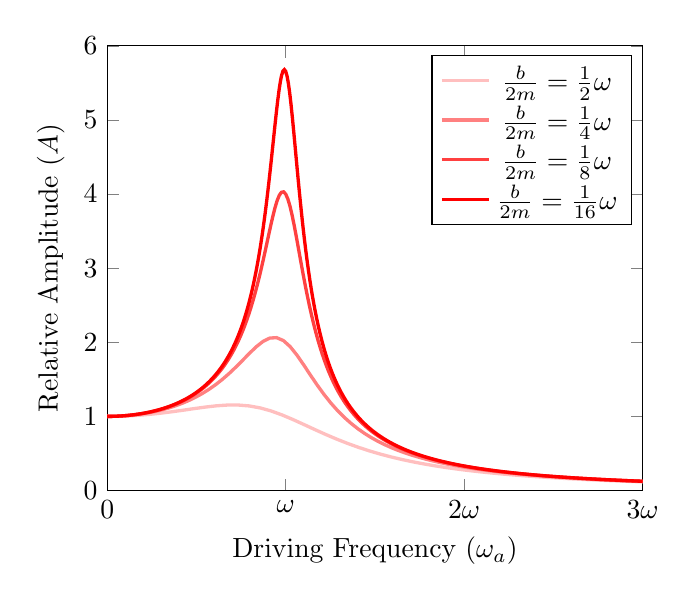
\begin{tikzpicture}
    \begin{axis}[
        width=3.3in,
        xmin=0,xmax=3, xlabel=Driving Frequency ($\omega_a$),
        xtick={0,1,2,3}, xticklabels={0,$\omega$,$2\omega$,$3\omega$},
        ymin=0,ymax=6, ylabel=Relative Amplitude ($A$),
        ytick={0,1,2,3,4,5,6}
      ]
      \addplot[
        color=red!25,
        samples=50,
        domain=0:3,
        very thick]{1/sqrt((1-x^2)^2+x^2)};
      \addlegendentry{$\frac b{2m}=\frac12\omega$}
      \addplot[
        color=red!50,
        samples=80,
        domain=0:3,
        very thick]{1/sqrt((1-x^2)^2+x^2/4)};
      \addlegendentry{$\frac b{2m}=\frac14\omega$}
      \addplot[
        color=red!75,
        samples=250,
        domain=0:3,
        very thick]{1/sqrt((1-x^2)^2+x^2/16)};
      \addlegendentry{$\frac b{2m}=\frac18\omega$}
      \addplot[
        color=red,
        samples=400,
        domain=0:3,
        very thick]{1/sqrt((1-x^2)^2+x^2/32)};
      \addlegendentry{$\frac b{2m}=\frac1{16}\omega$}
    \end{axis}
  \end{tikzpicture}
  \caption{Amplitude response to the driving frequency $\omega_a$.}
  \label{fig:amp-response}
\end{figure}
Plotting amplitude $A$ as a function of driving frequency $\omega_a$ shows
that, for a lightly damped system (i.e.\ small $b$), resonance response is
highest when $\omega_a\approx\omega\approx\omega$, and that smaller the
damping constant $b$, the higher and narrower the peak is.

The phase constant $\phi$ in Eq.\ref{eq:gen-solution3} also depends on the
driving frequency $\omega_a$.
\begin{equation}
  \boxed{\tan\phi=\frac{b\omega_a}{m(\omega^2-\omega_a^2)}}
\end{equation}
When $\omega_a=\omega$ is substituted into the phase shift expression, the
right-hand side becomes undefined. From this, we obtain a phase shift of
$\phi=\pi/2$. Taking derivative of $x(t)$ for velocity $v(t)$, and
substituting $\phi=\pi/2$:
\begin{equation}
  v(t)=\dot x
  =-A\omega_a\sin(\omega_a t-\frac{\pi}2)
  =A\omega_a\cos(\omega_a t)
\end{equation}
At resonance, the object is always moving in the same direction as the
driving force:
\begin{align*}
  v(t)&=A\omega_a\cos(\omega_a t)\\
  F_a(t)&=F\cos(\omega_a t)
\end{align*}
This also makes sense from a work-energy perspective, because now the
external force is doing positive work to the system.

\textbf{Resonance} is caused by in-phase excitation near the natural
frequency. This means that the frequency of the driving force is
\emph{approximately} equal to the natural frequency of the damped oscillator:
\begin{equation}
  \omega_a=\sqrt{\omega^2-\frac{b^2}{2m^2}}
  \quad\text{where}\quad\omega=\sqrt{\frac km}
\end{equation}
For a lightly damped system, $\omega_a\approx\omega\approx\omega$. Also, the
driving force follows the motion of the oscillator.
